\section{Hyperparameters}
\label{app:hyper}

\begin{table}[h]
\centering
\small
\caption{The released recipe. The original recipe is identical minus the ``later-iteration training'' block.}
\begin{tabular}{@{}p{4.6cm}p{10.9cm}@{}}
\toprule
\multicolumn{2}{@{}l}{\emph{Model}} \\
Tokens & 81 cells; input one-hot over 10 symbols; output 9 logits per cell \\
Blocks per iteration & 4, pre-norm, weights shared across iterations \\
Width, heads, feed-forward width & 128, 4, 512 (ReLU) \\
Position & 2D rotary embedding on queries and keys, 16 dimensions per axis, base 10 \\
Dropout & 0.1 (attention, residual branches, feed-forward) \\
State between iterations & previous state plus a linear map of the predicted probabilities; no normalization \\
Parameters & 796,937 \\
\midrule
\multicolumn{2}{@{}l}{\emph{Optimization}} \\
Loss & cross-entropy on empty cells, averaged over 16 iterations \\
Optimizer & AdamW, $\beta=(0.9, 0.95)$, weight decay 0.01, no gradient clipping \\
Learning rate & \lr{2} peak, 1,400-step linear warmup, cosine decay to 1\% of peak \\
Batch size, steps & 2048, 50,000 (20,000 with a 560-step warmup for the short schedule) \\
Precision & BF16 autocast with compiled model during training \\
Training pool & first 2.7M puzzles of the Sudoku-Extreme training split \\
Pool by step & rated 51+ (281K puzzles) to 10K; 11+ (1.64M) to 20K; 1+ (2.31M) to 30K; all to 50K \\
\midrule
\multicolumn{2}{@{}l}{\emph{Later-iteration training}} \\
Share of batches & 20\%, chosen independently per batch \\
Gradient-free iterations & drawn uniformly from $\{32, 64, 128, 256, 512\}$; dropout on \\
Loss & on the 16 iterations that follow, same loss; replaces the standard iterations 1--16 on those batches \\
\midrule
\multicolumn{2}{@{}l}{\emph{Inference}} \\
Precision & FP32, TensorFloat-32 disabled, batch size 256 \\
Iterations & 1024 unless stated; no early stopping, damping or answer selection \\
\bottomrule
\end{tabular}
\end{table}

\section{The six new training runs}
\label{app:cohort}

The six runs marked ``new'' in \tabref{tab:late} were trained on 19 November 2026 from the repository's unmodified code (PyTorch 2.10, one H200 GPU each), using three seeds fixed beforehand, with every started run reported.

\begin{table}[h]
\centering
\small
\caption{The six new runs. ``Best checkpoint'' and ``Final'' report FP32 accuracy (\%) at 1024 iterations on 1,000 benchmark puzzles across the 50 checkpoints saved every 1,000 steps. The last column counts how many of the 25,000 benchmark puzzles the final checkpoint solves at some iteration up to 4096 and later gets wrong.}
\label{tab:cohort}
\begin{tabular}{@{}llrrrr@{}}
\toprule
Recipe & Seed & Best checkpoint & at step & Final & Solved, then lost \\
\midrule
Later-iteration training & 20261119 & 98.7 & 45K & 98.6 & 166 \\
Later-iteration training & 20261120 & 98.2 & 37K & 97.4 & 4,155 \\
Later-iteration training & 20261121 & 98.5 & 42K & 97.2 & 950 \\
\midrule
Original recipe & 20261119 & 97.3 & 25K & 2.6 & 24,584 \\
Original recipe & 20261120 & 99.1 & 35K & 80.5 & 8,109 \\
Original recipe & 20261121 & 62.8 & 3K & 0.8 & 24,676 \\
\bottomrule
\end{tabular}
\end{table}

\paragraph{Checkpoint selection.} Selecting each original-recipe run's best checkpoint would yield 97.3\%, 99.1\%, and 62.8\%, against 2.6\%, 80.5\%, and 0.8\% for the final ones. With later-iteration training, the best checkpoint is within 1.3 points of the final one in every run.

\paragraph{The run that fades at 4096 iterations.} Later-iteration seed 20261120 drops from 97.5\% at 1024 iterations to 83.9\% at 4096, losing 11\% to 15\% of puzzles in every difficulty bucket including the easiest. Its state stays much smaller than in its sibling runs: at iteration 1024, median state RMS is 97 compared to 415 and 736. Meanwhile, the median margin in a puzzle's weakest cell erodes steadily from 15.5 logits at iteration 16 to 5.5 at 1024 and 2.0 at 4096, whereas the other two runs hold between 9 and 11. This looks like the drift analyzed in \secref{sec:analysis}, moving more slowly. We saw one such run and haven't tested whether wider starting offsets prevent it.

\section{Training on 1,000 puzzles}
\label{app:small}

HRM and TRM train on 1,000 puzzles expanded into 1,000 symmetry-augmented copies each, reporting 55.0\% and 87.4\% on the full test split \citep{wang2025hierarchical,jolicoeur2025less}. We ran our model in this regime, with relabeled digits, row and column permutations within and across bands, and random transposes as the augmentations.

\begin{table}[h]
\centering
\small
\caption{Our model trained on 1,000 puzzles: full-test-split accuracy (\%) in FP32. Multi-run rows report min--max across runs. The four runs in the second-to-last row span three seeds plus a second random sample of 1,000 puzzles.}
\label{tab:small}
\begin{tabular}{@{}lrlrrrrr@{}}
\toprule
 & & & & & \multicolumn{3}{c}{Inference iterations} \\
\cmidrule(l){6-8}
Difficulty sampling & Steps & Recipe & Weight decay & Runs & 16 & 128 & 1024 \\
\midrule
Hardest first & 50K & Original & 0.01 & 1 & 9.4 & 2.8 & 0.0 \\
Hardest first & 50K & Later-iteration & 0.01 & 1 & 13.0 & 14.1 & 10.6 \\
All from the start & 50K & Original & 0.01 & 1 & 20.9 & 16.4 & 0.0 \\
All from the start & 50K & Later-iteration & 0.01 & 1 & 22.7 & 22.0 & 18.9 \\
\midrule
All from the start & 10K & Original & 0.01 & 1 & 45.3 & 42.6 & 0.3 \\
All from the start & 10K & Original & 1.0 & 1 & 42.8 & 52.7 & 44.8 \\
All from the start & 10K & Later-iteration & 0.01 & 4 & 47.2--48.9 & 50.1--51.7 & 46.3--51.6 \\
All from the start & 10K & Later-iteration & 0.3 & 3 & 47.4--51.4 & 52.4--57.1 & 52.3--57.1 \\
\bottomrule
\end{tabular}
\end{table}

Left unmodified, both recipes memorize the 1,000 puzzles (\tabref{tab:small}). Sampling all difficulties from step 0 and cutting the schedule to 10,000 steps (a length we picked by inspecting test accuracy) recover most of the gap: later-iteration training then solves 46\% to 57\% at 1024 iterations across seven runs, matching HRM while trailing TRM by a wide margin.

\section{Additional figures}
\label{app:gallery}

\begin{figure}[H]
\centering
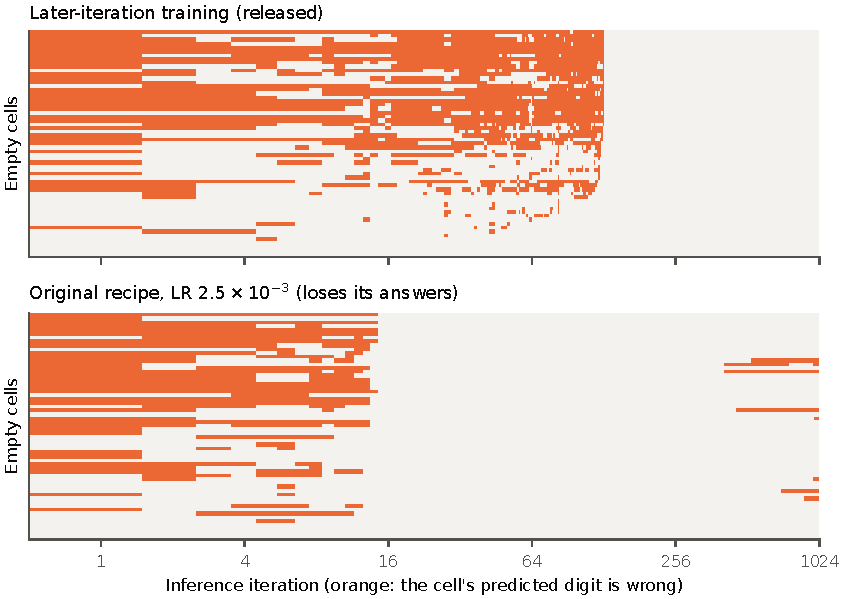
\includegraphics[width=0.76\linewidth]{cell_timeline}
\caption{The puzzle from \figref{fig:board} in two checkpoints. Each row is an empty cell, shaded orange on iterations where its prediction is wrong. \emph{Top:} the released checkpoint flips cells back and forth before solving the puzzle at iteration 130 and holding it. \emph{Bottom:} a failing original-recipe checkpoint solves the puzzle at iteration 15 and holds it until iteration 407, after which cells peel off one by one.}
\label{fig:timeline}
\end{figure}

\begin{figure}[H]
\centering
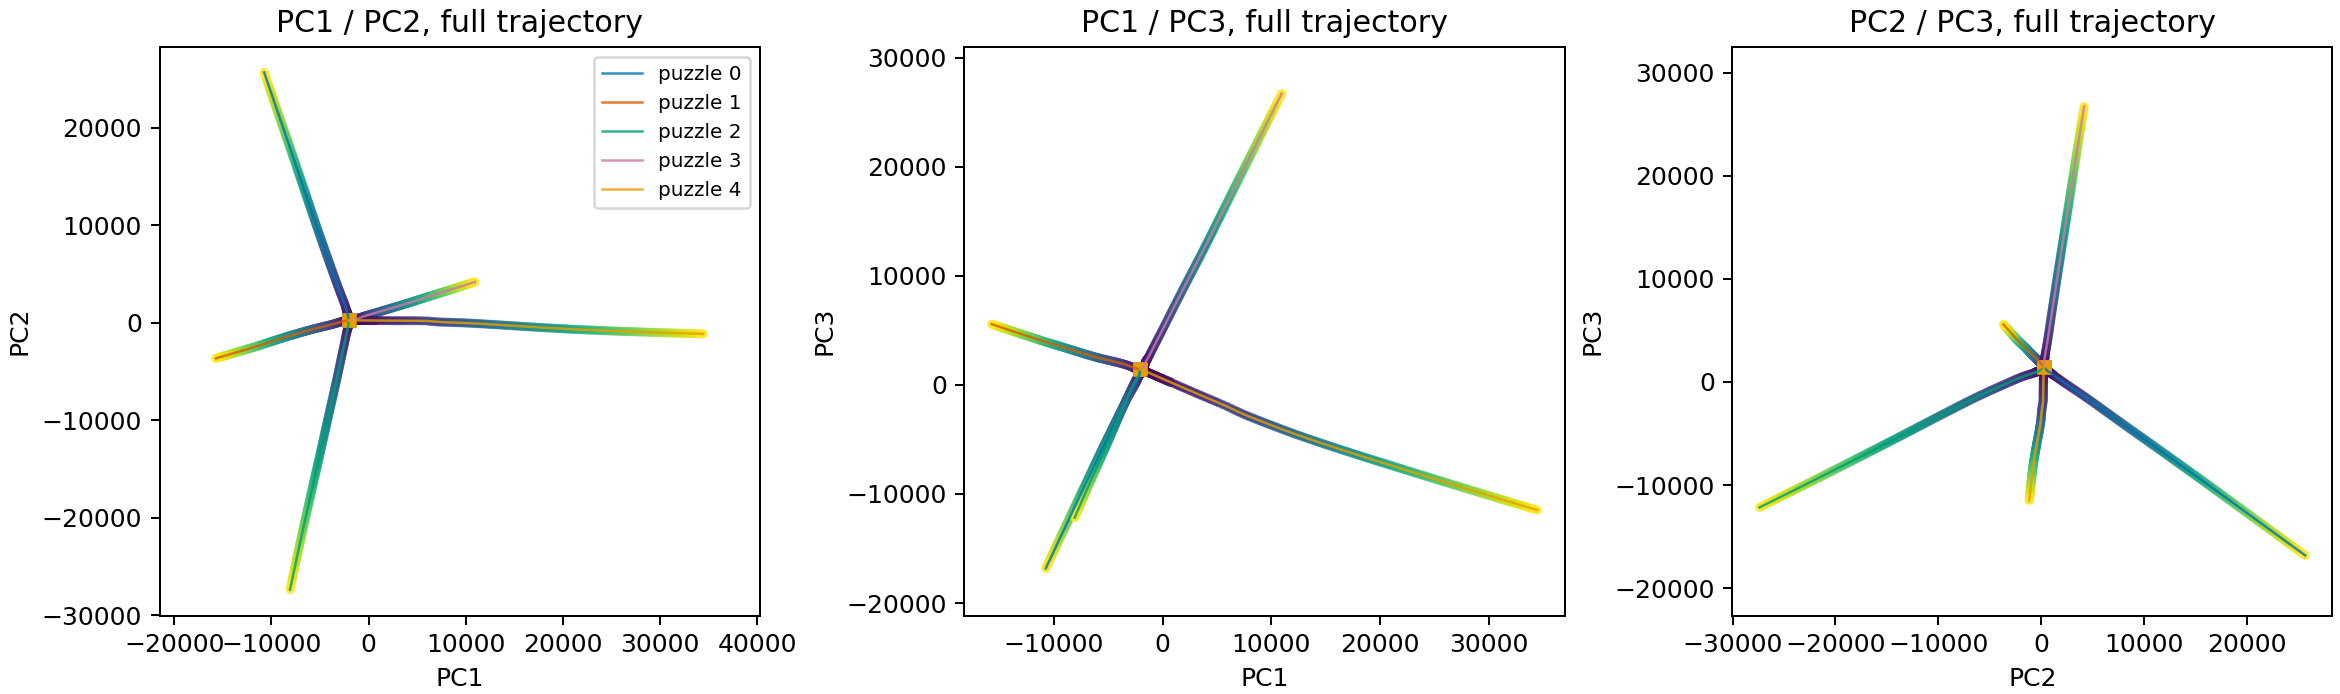
\includegraphics[width=\linewidth]{repo_state_pca}
\caption{State trajectories of five puzzles over 1,024 iterations in a shared PCA basis, colored from early (purple) to late (yellow), for a later-iteration checkpoint. Each puzzle traces a nearly straight ray corresponding to the linear norm growth in \secref{sec:analysis}.}
\label{fig:pca}
\end{figure}

\begin{figure}[H]
\centering
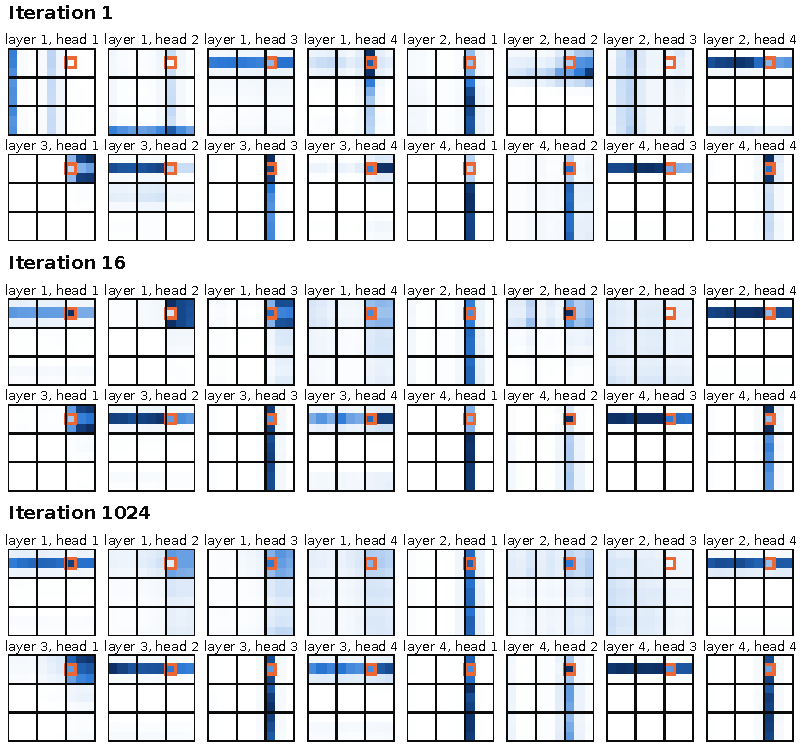
\includegraphics[width=\linewidth]{attention_all_heads}
\caption{All 16 attention heads of the released checkpoint at iterations 1, 16, and 1024. Each grid shows mean attention from the outlined cell over 1,000 puzzles on its own color scale. At iteration 1, several heads attend to rows or columns other than the cell's own. By iteration 16, the row, column, and box heads of \figref{fig:attention} have emerged, and they stay largely unchanged through iteration 1024.}
\label{fig:allheads}
\end{figure}

\begin{figure}[H]
\centering
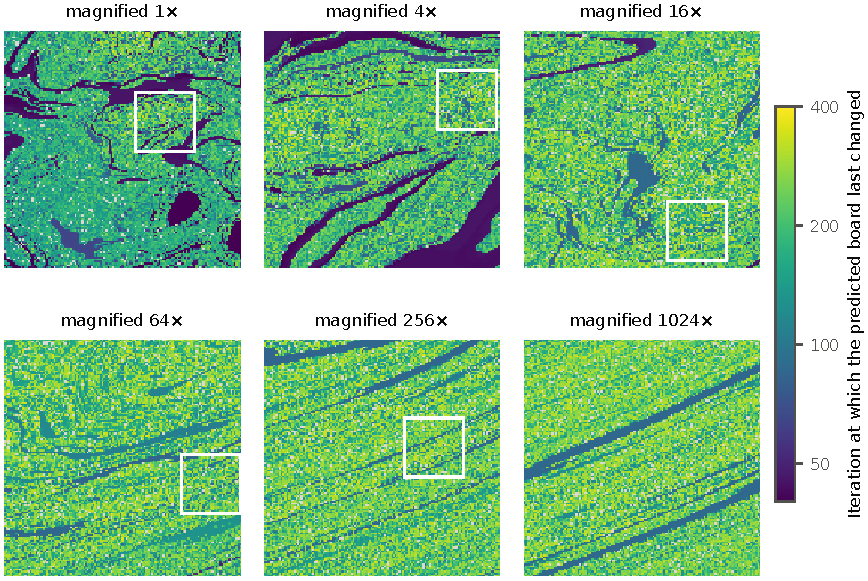
\includegraphics[width=0.88\linewidth]{perturbation_maps}
\caption{Nearby starting states can settle at very different iterations. Starting from a puzzle that an accurate 20K-step model solves slowly, we perturb $h_0$ along two random directions and run 2,048 FP64 iterations from a $129\times129$ grid of starts. Color marks the last iteration where the predicted board changed; grey marks the 2--6\% of starts that never landed on the right board. Each panel zooms into the white box of the previous one, and fine bands persist at $1,024\times$ magnification. For a puzzle solved in two iterations, the map is a single flat color.}
\label{fig:maps}
\end{figure}

\begin{figure}[H]
\centering
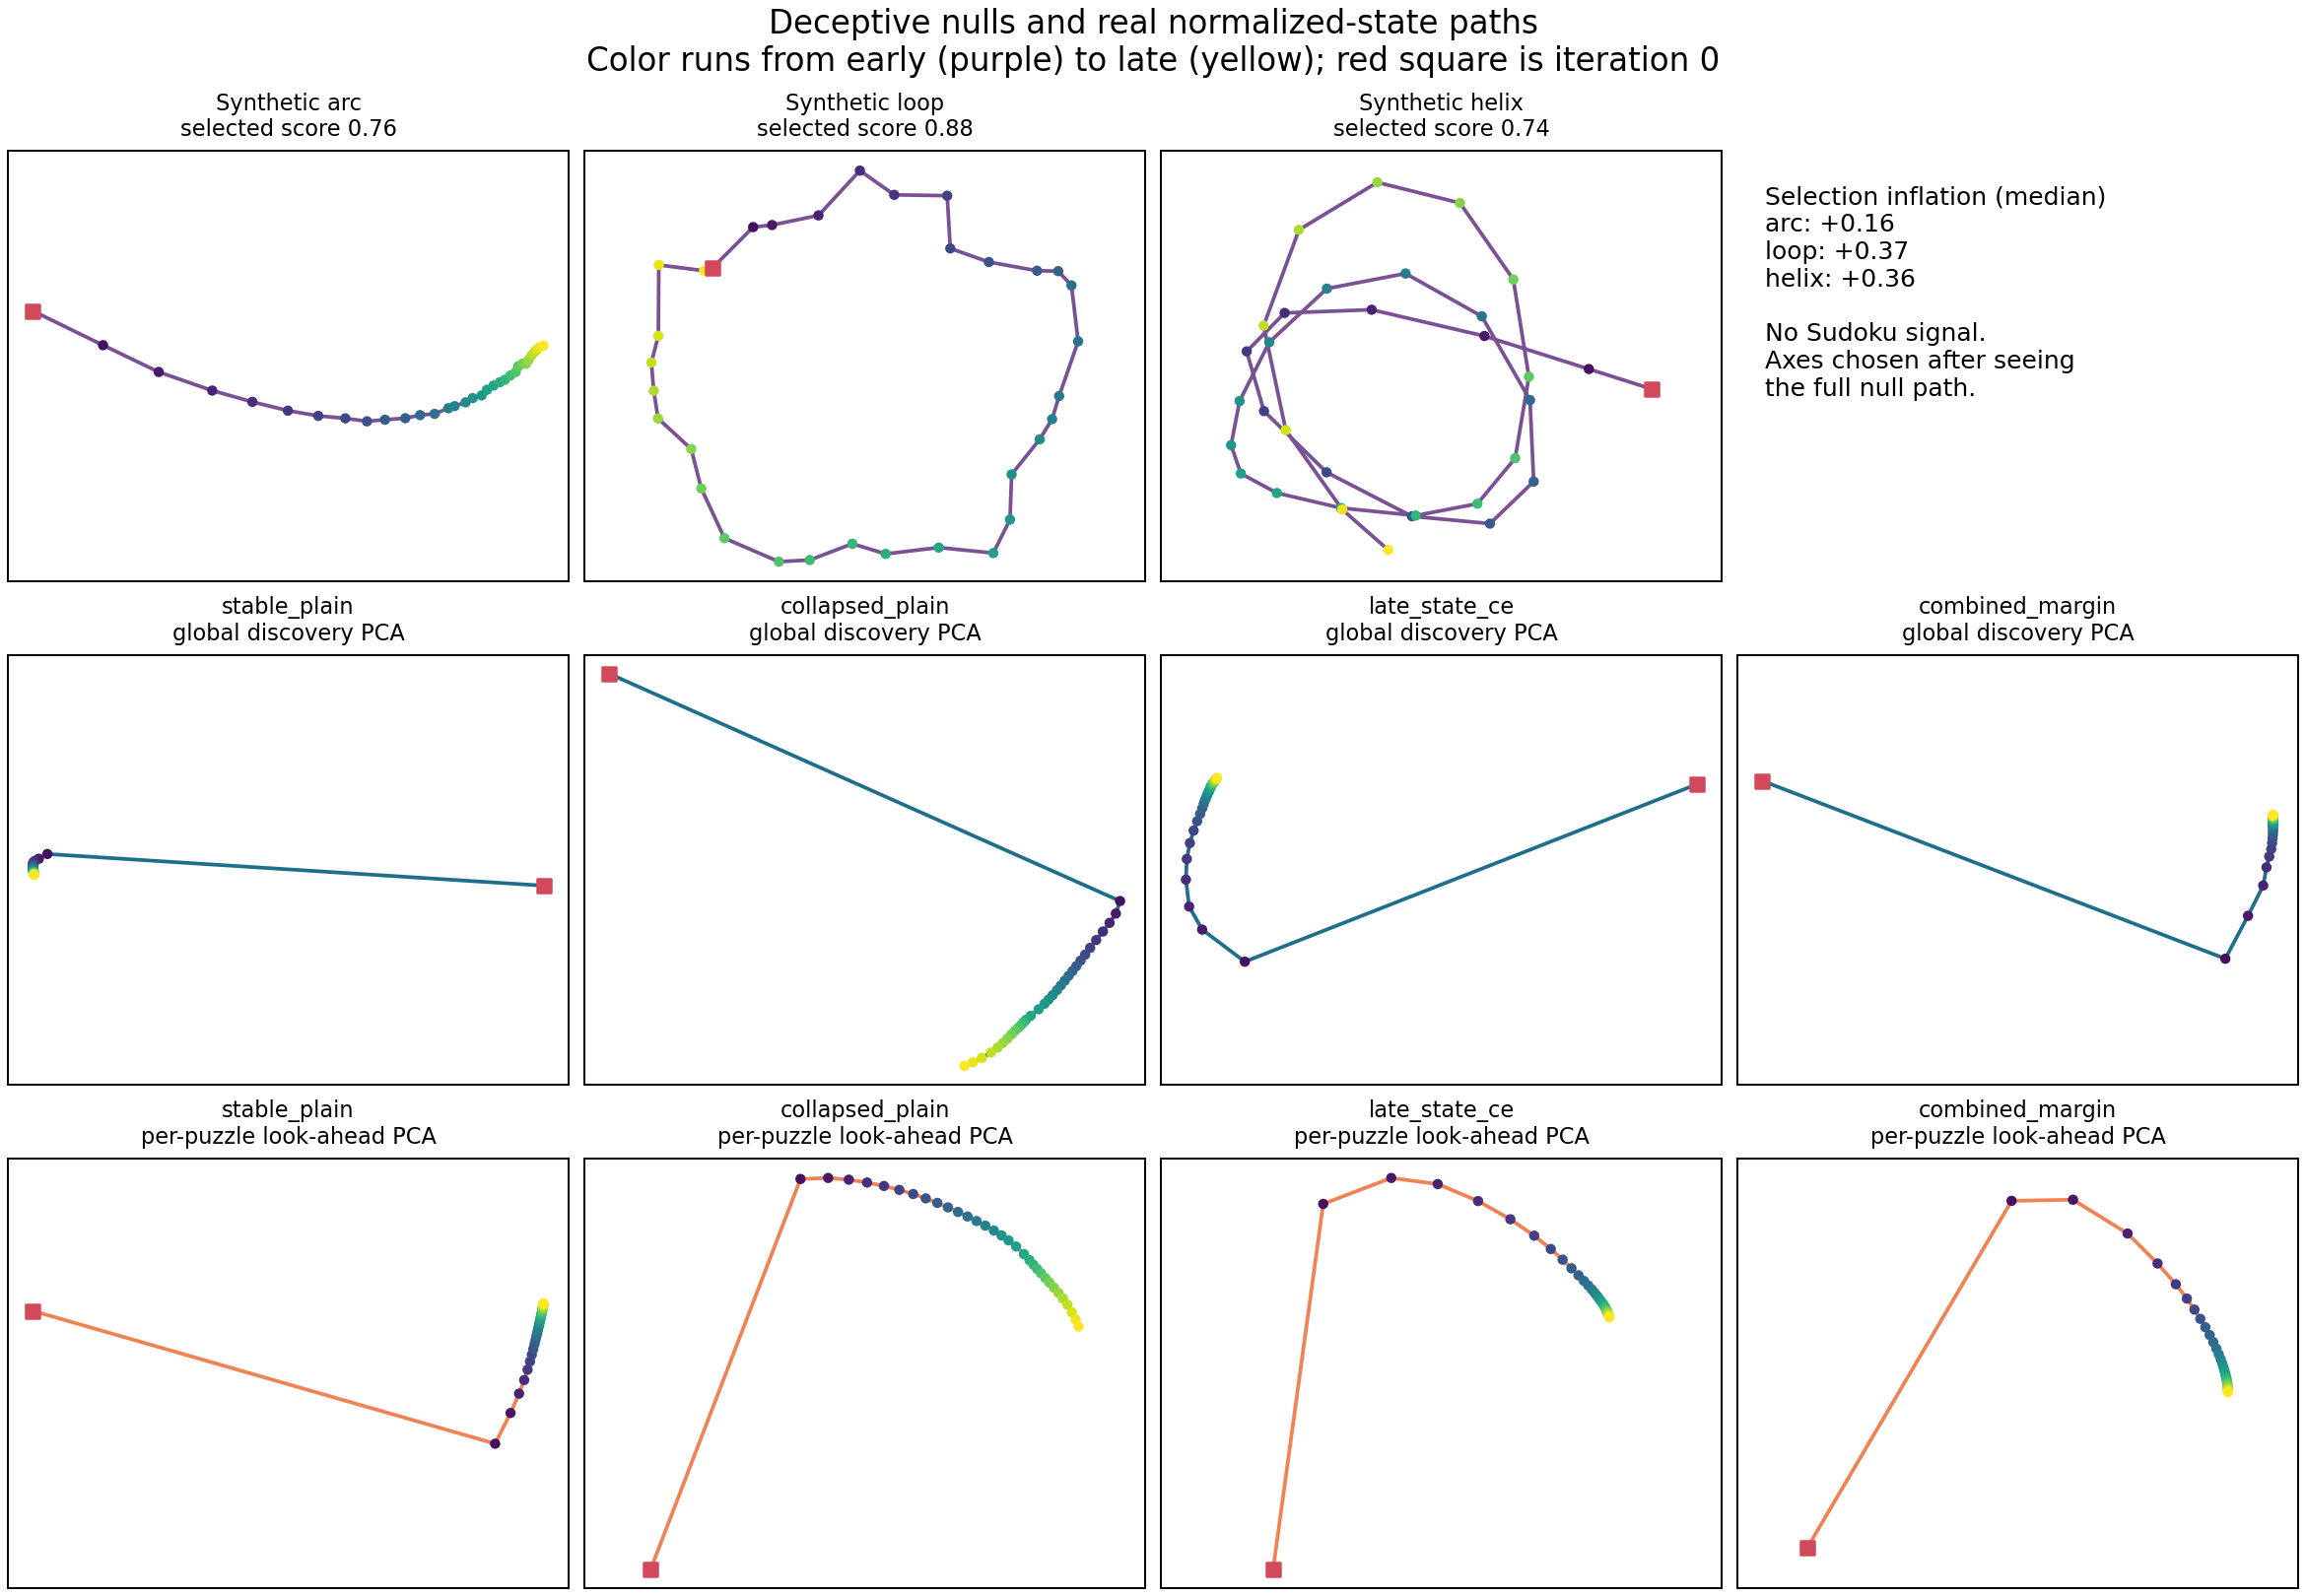
\includegraphics[width=0.70\linewidth]{repo_adversarial_gallery}
\caption{Why we stopped trusting trajectory projections. \emph{Top row:} random smooth curves with no Sudoku signal, each projected to maximize an arc, loop, or helix score. \emph{Other rows:} real trajectories, normalized to unit length, under a shared PCA basis and a per-puzzle basis. Labels use internal repository names: \texttt{stable\_plain} (accurate original-recipe checkpoint), \texttt{collapsed\_plain} (failing original-recipe checkpoint), \texttt{late\_state\_ce} (later-iteration training), and \texttt{combined\_margin} (adds a second window and late margin term).}
\label{fig:gallery}
\end{figure}

\section{Repository guide}
\label{app:repo}

The repository (\url{https://github.com/chenglou/sotaku}) contains full writeups for every experiment summarized here without a table; its README indexes them under ``Research Notes''. The main files are:

\begin{itemize}
\raggedright
\item \path{STALE_EXPERIMENTS_DOC.md}: the early design history in the order it happened, about two hundred experiments. \path{pos_embedding/EXPERIMENTS_POS.md}, \path{cosine/EXPERIMENTS_COSINE.md}, \path{muon/EXPERIMENTS_MUON.md} and \path{rrn/RRN_EXPERIMENTS.md} cover position encodings, the learning-rate schedule, Muon and the recurrent relational network.
\item \path{iters/EXPERIMENTS_ITERS.md}: accuracy at large iteration counts, the February and July runs, and the single runs with other learning rates, batch sizes and widths.
\item \path{looping/EXPERIMENTS_LOOPING.md}: later-iteration training, including the 20K-step runs, second windows, margin terms and damping at inference.
\item \path{stabilize/EXPERIMENTS_STABILIZE.md}: normalizing the state and the other attempts to stabilize the original recipe.
\item \path{es/EXPERIMENTS_ES.md}: evolution strategies, plus the pixel-input and maze variants of the task.
\item \path{looping/weight_tying/RESULTS.md}, \path{looping/window_selection/RESULTS.md}, \path{looping/width_50k/README.md}, \path{looping/hyperloop_50k/RESULTS.md} and \path{looping/attention_residuals/RESULTS.md}: shared against separate weights with the fresh puzzle set, the choice of starting points, width 160, the extra gated states, and the Inkling 2 Mini loop design.
\item \path{looping/trajectory_viz/study/README.md}, \path{looping/spectral_diagnostics/RESULTS.md} and \path{looping/basin_diagnostics/RESULTS.md}: the readout study and projection controls, the corrected Jacobian analysis, and the perturbation maps.
\item \path{release/PRECISION_RESULTS.md}: the inference-precision table. \path{paper/README.md}: how to rebuild this paper's tables and figures.
\end{itemize}
